\chapter{The RAW Dataset}\label{ch:benchmarks_and_metrics}
In this chapter the RAW dataset is going to be presented. This dataset has been produced as a requirement of the FlexSight\footnote{http://www.flexsight.eu/} project. FlexSight is a research project founded by the European Community's project ECHORD++\footnote{http://echord.eu/}.  This project involves three main partners: the Ro.Co.Co. Laboratory\footnote{http://www.dis.uniroma1.it/~labrococo/} of DIAG (Department of Computer, Control, and Management Engineering  Antonio Ruberti at Sapienza University of Rome), which provides expertise in software design and development for robotic perception applications; IT+Robotics\footnote{http://www.it-robotics.it/}, which provides expertise in the industrial robotics domain; and Robox\footnote{http://www.robox.it/en-US/}, a company specialized in the development of innovative hardware and software solutions for robotics and control systems. 

More details about the FlexSight project can be found in the Appendix \ref{apx:flexsight} of this thesis.

\section{RAW Dataset Features}\label{sec:raw_features}
As like as the previous datasets presented in sections \ref{subsec:mvtex_itodd} and \ref{subsec:tless_dataset} also the RAW Dataset has been built for industrial scenarios. The main scope of the RAW Dataset is to build a large and consistent test bed for texture-less object detection and localization algorithms. The name of the dataset is related to the RoboCup@Work competition, which more details are given in the Appendix \ref{apx:robocupatwork}, and it contains all the objects used in the robotic competition plus other objects from other past robotics events, such as the RoCKIn@Work\footnote{http://rockinrobotchallenge.eu/} (Robot Competitions Kick Innovation in Cognitive Systems and Robotics) and ERL\footnote{https://www.eu-robotics.net/robotics\_league/index.html} (European Robotics League). 

As already mentioned, all the objects present in the dataset are texture-less objects and are inspired to the industrial settings, e.g. parts of a motor, bearings, nuts, motor axis and others. A compact view of all the objects present in the dataset is given in Figure \ref{fig:raw_obj_examples}, and the complete list of objects with their specific name and class is reported in Table \ref{tab:raw_objs_list}.

\begin{table}
    \centering
    \begin{tabular}{| l | l | l |}
    \hline
    \textbf{Name} & \textbf{Class} & \textbf{Description} \\ \hline
    F20\_20\_B & 0 & Black small aluminium profile \\
    F20\_20\_G & 1 & Gray small aluminium profile \\
    M20 & 2 & Small nut \\
    M20\_100 & 3 & Heavy large screw \\
    M30 & 4 & Big nut \\
    R20 & 5 & Plastic tube with shaped borders \\
    S40\_40\_B & 6 & Black large aluminium profile \\
    S40\_40\_G & 7 & Gray large aluminium profile \\
    V20 & 8 & Plastic tube without shaped borders \\
    Bearing\_box & 9 & Small motor box for bearings \\
    Bearing\_box\_B & 10 & Small motor box for bearings (Type B) \\
    Motor & 11 & Black plastic reconstruction of a motor \\
    Axis & 12 & Aluminium motor axis \\
    Distance\_tube & 13 & Small aluminium ring \\
    Bearing & 14 & Real bearing for motors \\
    Cover\_plate\_NOHOLE & 15 & Thin aluminium plate with hole \\
    Cover\_plate\_HOLE & 16 & Thin aluminium plate without hole \\
    Cover\_plate\_BOX & 17 & Black plastic box for cover plates \\
    Bearing\_box\_BOX & 18 & Black plastic box for bearing boxes \\
    \hline
    \end{tabular}
    \caption{\textbf{The RAW Dataset Objects.} In this table is reported the list of all the objects present in the RAW dataset, with their name and class.}
    \label{tab:raw_objs_list}
\end{table}

\begin{figure}
    \centering
    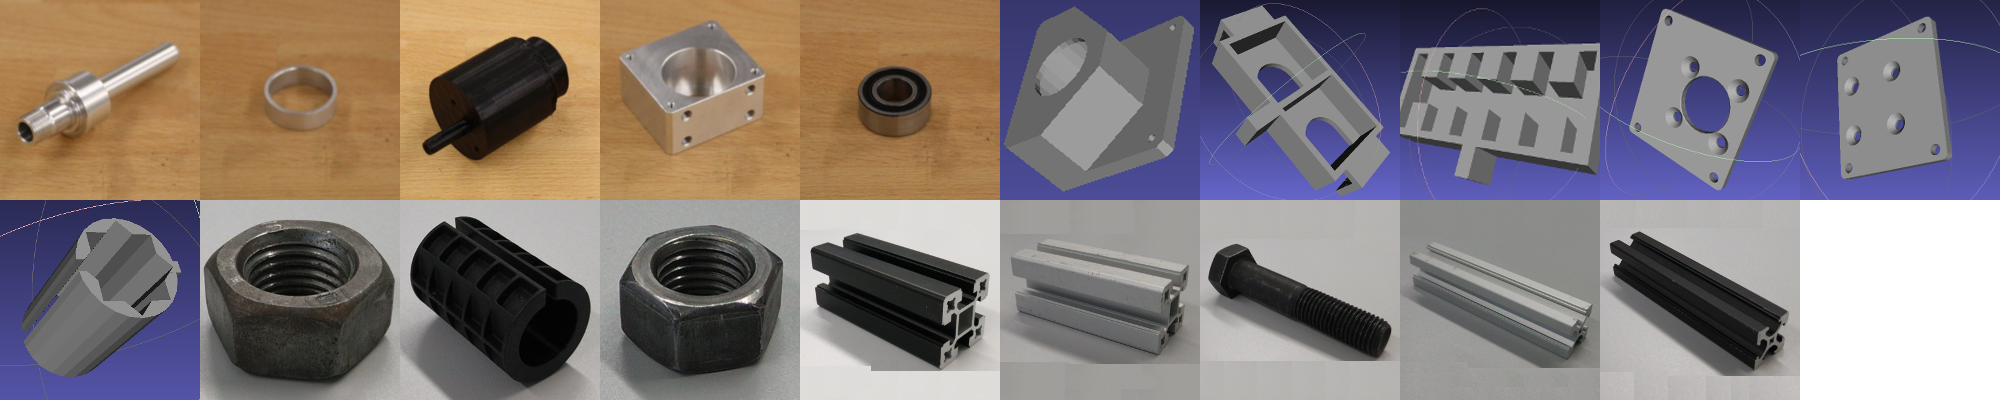
\includegraphics[width=0.9\textwidth]{figures/3_raw_dataset/raw_obj_examples}
    \caption{\textbf{RAW Dataset Objects.} A compact view of all the 19 classes of objects present in the RAW Dataset.}
    \label{fig:raw_obj_examples}
\end{figure}

The main features of this dataset are the following:
\begin{itemize}
	\item \textbf{19 indutry relevant objects}: no discriminative color, no texture, often similar in shape;
	\item \textbf{3 different sensors}: FlexSight sensor, Microsoft Kinect2, Intel RealSense SR-300;
	\item \textbf{Test images (7K from each sensor)}: originated from 15 test scenes. The scene complexity varies from simple scenes with several isolated objects to very challenging ones with multiple object instances and a high amount of clutter and occlusion. Images include: RGB and Depth for Kinect2 and RealSense SR-300; 2 grey-scale images (with and without projected laser pattern) for the FlexSight sensor;
	\item \textbf{19 object 3D CAD models}: all the objects have a specific 3D CAD model.
\end{itemize}

Each image of the dataset comes with ground truth estimate of all the objects present in the scene. The full 3D position in space, rotation plus translation with respect to the camera frame, has been annotated with a specific protocol that involved both manually intervention of the user by means of our own developed labeling tool and some other automatic procedures for propagating the pose in a given reference frame to all the other images of the dataset.

\begin{figure}
    \centering
    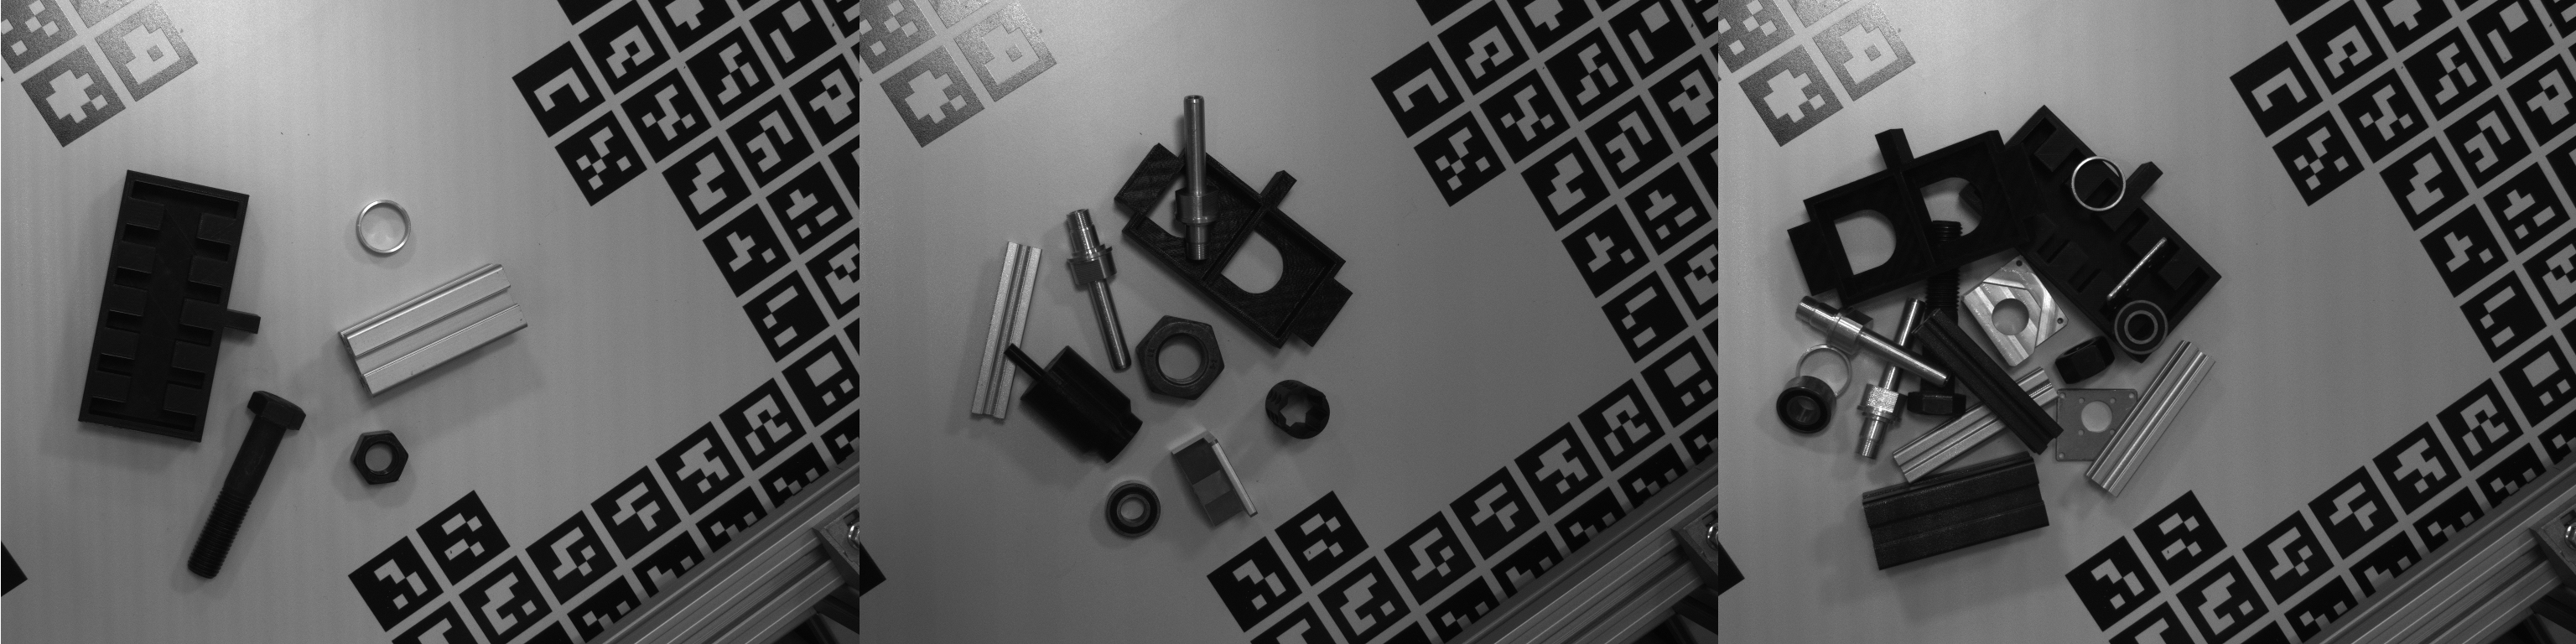
\includegraphics[width=0.9\textwidth]{figures/3_raw_dataset/easy_medium_hard_scene}
    \caption{\textbf{RAW Dataset Scenes Comparison.} From left to right: easy scene, medium scene and hard scene. All the images refers to the camera left of the FlexSight sensor and are without the projected laser pattern.}
    \label{fig:easy_medium_hard_scene}
\end{figure}

\section{Details of the Scenes}\label{sec:raw_scenes_details}
As already anticipated, the RAW Dataset comes with 15 different scenes. In particular, those scenes are aggregated in three different categories: \emph{easy}, \emph{medium} and \emph{hard}. This categorization depends on the level of complexity of the disposition of the objects in the scenes. An example of easy medium and hard scene comparison is given in Figure \ref{fig:easy_medium_hard_scene}. Moreover, easy scenes does not contain any occlusion or overlapping of the objects, while medium and hard scenes do.

Each scene is composed as follow:

\begin{itemize}
	\item \textbf{FlexSight Sensor Data}: 465 images, both for camera left and camera right of the sensor. Each image has been acquired with and without the projected laser pattern (See Figure \ref{fig:flexsight_laser_no_laser_ex}).
	\item \textbf{Microsoft Kinect 2}: 465 rgb-d images. We provide both rgb and depth image, together with the automatic generated registered pointcloud.
	\item \textbf{Intel Realsense SR300}: 465 rgb-d images. For the Intel Realsense SR300 only rgb and depth images are provided.
\end{itemize}

\begin{figure}
    \centering
    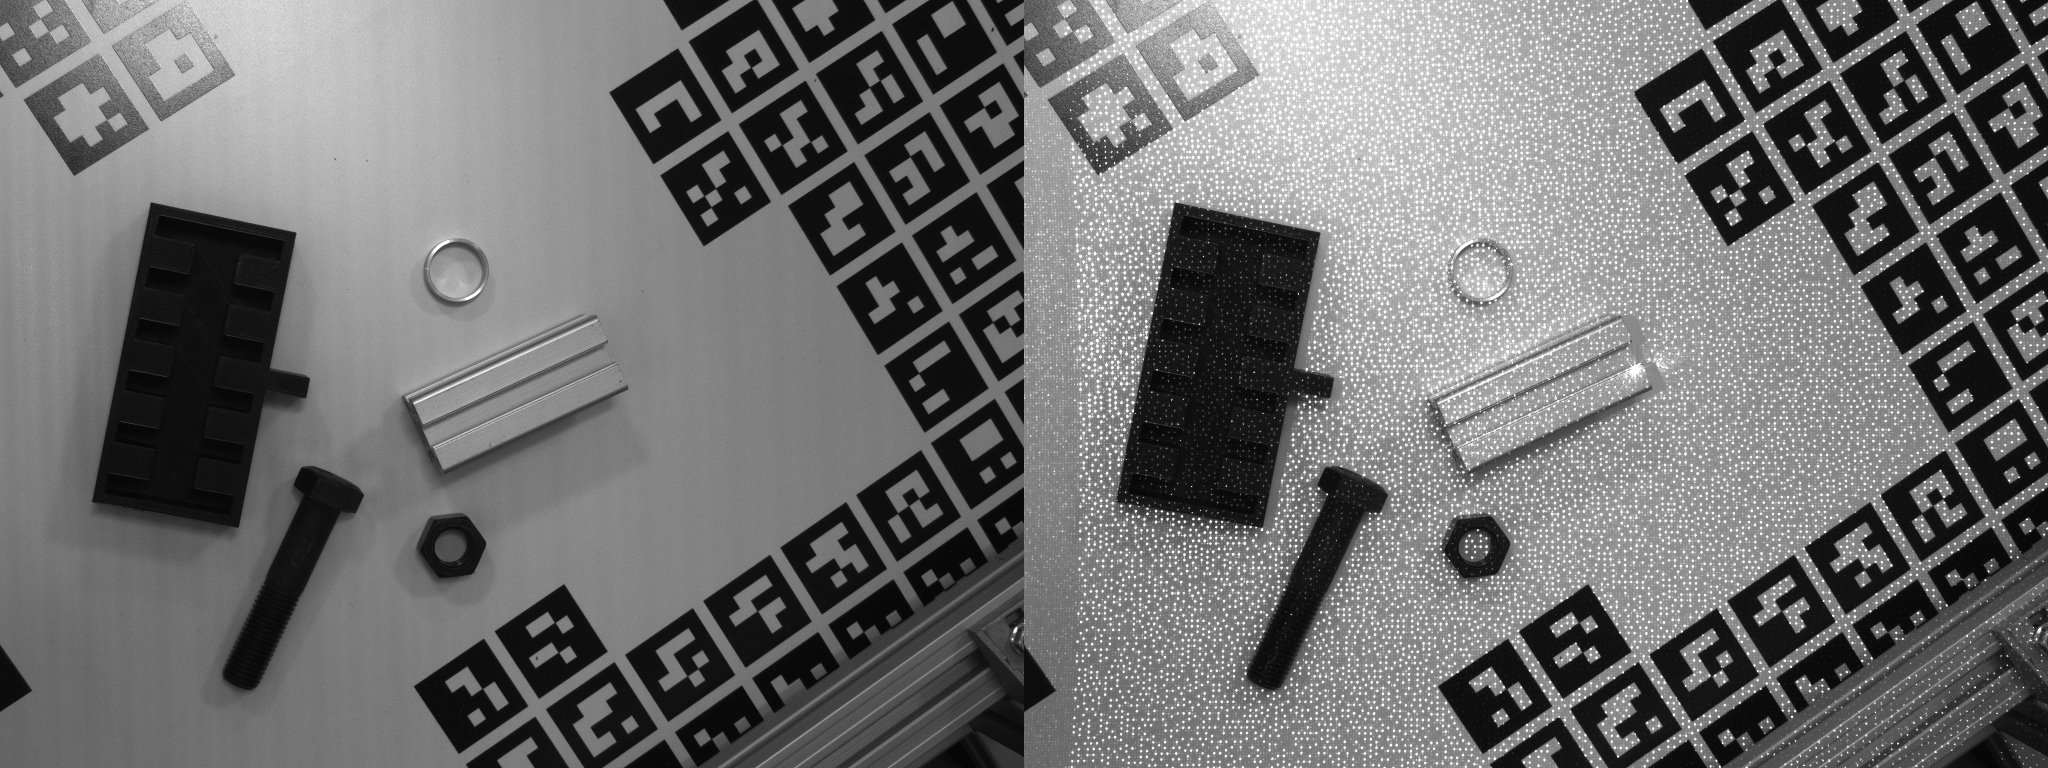
\includegraphics[width=0.9\textwidth]{figures/3_raw_dataset/flexsight_laser_no_laser_ex}
    \caption{\textbf{FlexSight Sensor Acquisition (with and without laser pattern).} On the left the FlexSight Sensor image acquired without projected laser pattern, on the right with projected laser pattern.}
    \label{fig:flexsight_laser_no_laser_ex}
\end{figure}

\section{Setup and Sensors}\label{sec:raw_setup_and_sensors}
To do ...

\section{Acquisition Procedure}\label{sec:raw_acquisition_procedure}
To do ...

\section{Ground Truth Estimation Protocol}\label{sec:ground_truth_estim}
To do ...

\subsection{Labelling tool}\label{subsec:raw_labeltool}
To do ...

\subsection{Pose Propagation Pipeline}\label{subsec:pose_propagation}
To do ...